\section{Project management}
A Trello board (Figure \ref{fig:trello}) has been used to keep track of weekly tasks, resources and issues. The tasks can be marked as "To-Do", "Doing" and "Done". This is reviewed in weekly meetings with the project supervisor and next week's tasks are decided on.

Progress is behind what would be expected if the original timeline had been restructured due to unavoidable personal issues arising and not putting in the hours per week as planned in the specification. A more organised weekly plan will be used to help with time management on the rest of the project and the scope of the project has been changed to allow for the lost time. The switch to using bare-metal code has made the software side considerably simpler and greatly increases the possible speed of development. Using Verilog to develop the hardware instead of Chisle reduces the learning curve allowing for development to start sooner.

\begin{figure}[H]
	\centering
	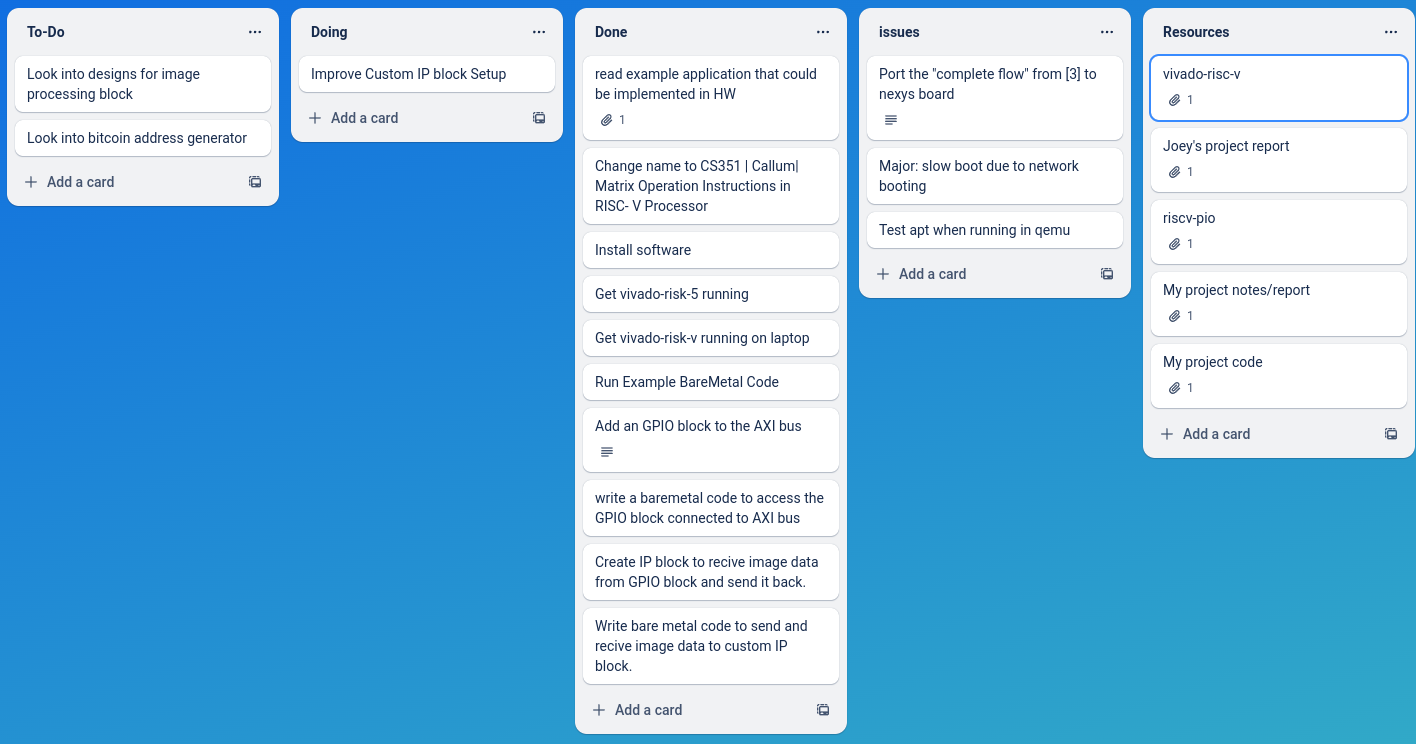
\includegraphics[scale=0.4]{trello}
	\caption{Current status of the project Trello board}
	\label{fig:trello}
\end{figure}

\section{Ethics}
This project does not require working with people and should not present any ethical issues. There should also be no legal issues as there is no intent to profit from this project.